\documentclass{../lab}

\labacronym{}
\labtitle{}

%\newcommand{\EnergyLossandStragglingof$\alpha$ParticlesinMetalFoils}{http://physics111.lib.berkeley.edu/Physics111/Reprints/RUT/01-Energy_Loss_and_Straggling.pdf}
%\newcommand{\ChamberandAlphaGunAssembly}{http://physics111.lib.berkeley.edu/Physics111/Reprints/RUT/RUT_Chamber_017.JPG}
%\newcommand{\HighEnergyData,VolumeII,}{http://physics111.lib.berkeley.edu/Physics111/Reprints/RUT/02-High_Energy_Particle_Data.pdf}
%\newcommand{\HowtomakeandmounttheGoldfoils}{http://physics111.lib.berkeley.edu/Physics111/Reprints/RUT/Procedure\%20for\%20Making\%20Foils.pdf}
%\newcommand{\RadiationSafety}{http://experimentationlab.berkeley.edu/RadiationSafety}
%\newcommand{\Physics111LibrarySite}{http://physics111.lib.berkeley.edu/Physics111/Reprints/RUT/RUT_index.html}
%\newcommand{\RutherfordDetector}{http://physics111.lib.berkeley.edu/Physics111/Reprints/RUT/RUT_Detector_018.JPG}

\begin{document}

\maketitle

\tableofcontents

\section{Rutherford Scattering Description (RUT)}

\begin{enumerate}
    \item \textbf{Note that there is NO eating or drinking in the 111-Lab anywhere, except in rooms 282 \& 286 LeConte on the bench with the BLUE stripe around it.} Thank You the Staff.

\end{enumerate}

An experiment that shook the world of physics was carried out by Rutherford in 1910. He found that when scattering alpha particles from gold foils, far more of them were scattered at large angles than were expected to by theory. He explained the finding by assuming that all of the mass and positive charge of an atom are concentrated in a small volume at the center, in a compact nucleus. He derived an equation in which the differential cross section for scattering by an atomic nucleus is proportional to the inverse fourth power of the sine of the scattering angle.

In this experiment the scattering formula is confirmed for the case of alpha particles scattered by gold nuclei in a thin gold foil. The charge on the gold nucleus will also be determined.

This experiment needs long counting times owing to the fact that only a small fraction of incident particles is scattered to large angles. The counting rate in the forward direction is on the order of $10^5$ particles/hr, while in the backward direction it is of the order of $10^{-1}$particles/hr! This makes the experiment difficult since background and electronic noise are larger than this. You set up the equipment and count, only returning to read out data and start another set. It's an easy experiment which requires patience. It is not a fun experiment, but instead illustrates the kind of work often needed to sort out one theory from another.

It is a good introduction to the electronics used in physics experiments (detectors, amplifiers, shapers, delay lines, pulse height analyzers, computer interfacing). Analyzing the data with a computer is necessary.

\begin{enumerate}
    \item Pre-requisites: None

    \item Days Allotted for the Experiment: 6

\end{enumerate}

This lab will be graded 20\% on theory, 30\% on technique, and 50\% on analysis. For more information, see the \href{\AdvancedLabSyllabus}{\textbf{Advanced Lab Syllabus}}.

Comments: E-mail \href{\MailDonOrlando}{\textbf{Don Orlando}}

\section{Rutherford Experiment Pictures}

\noindent
\href{http://experimentationlab.berkeley.edu/sites/default/files/images/RUT_3512.jpg}{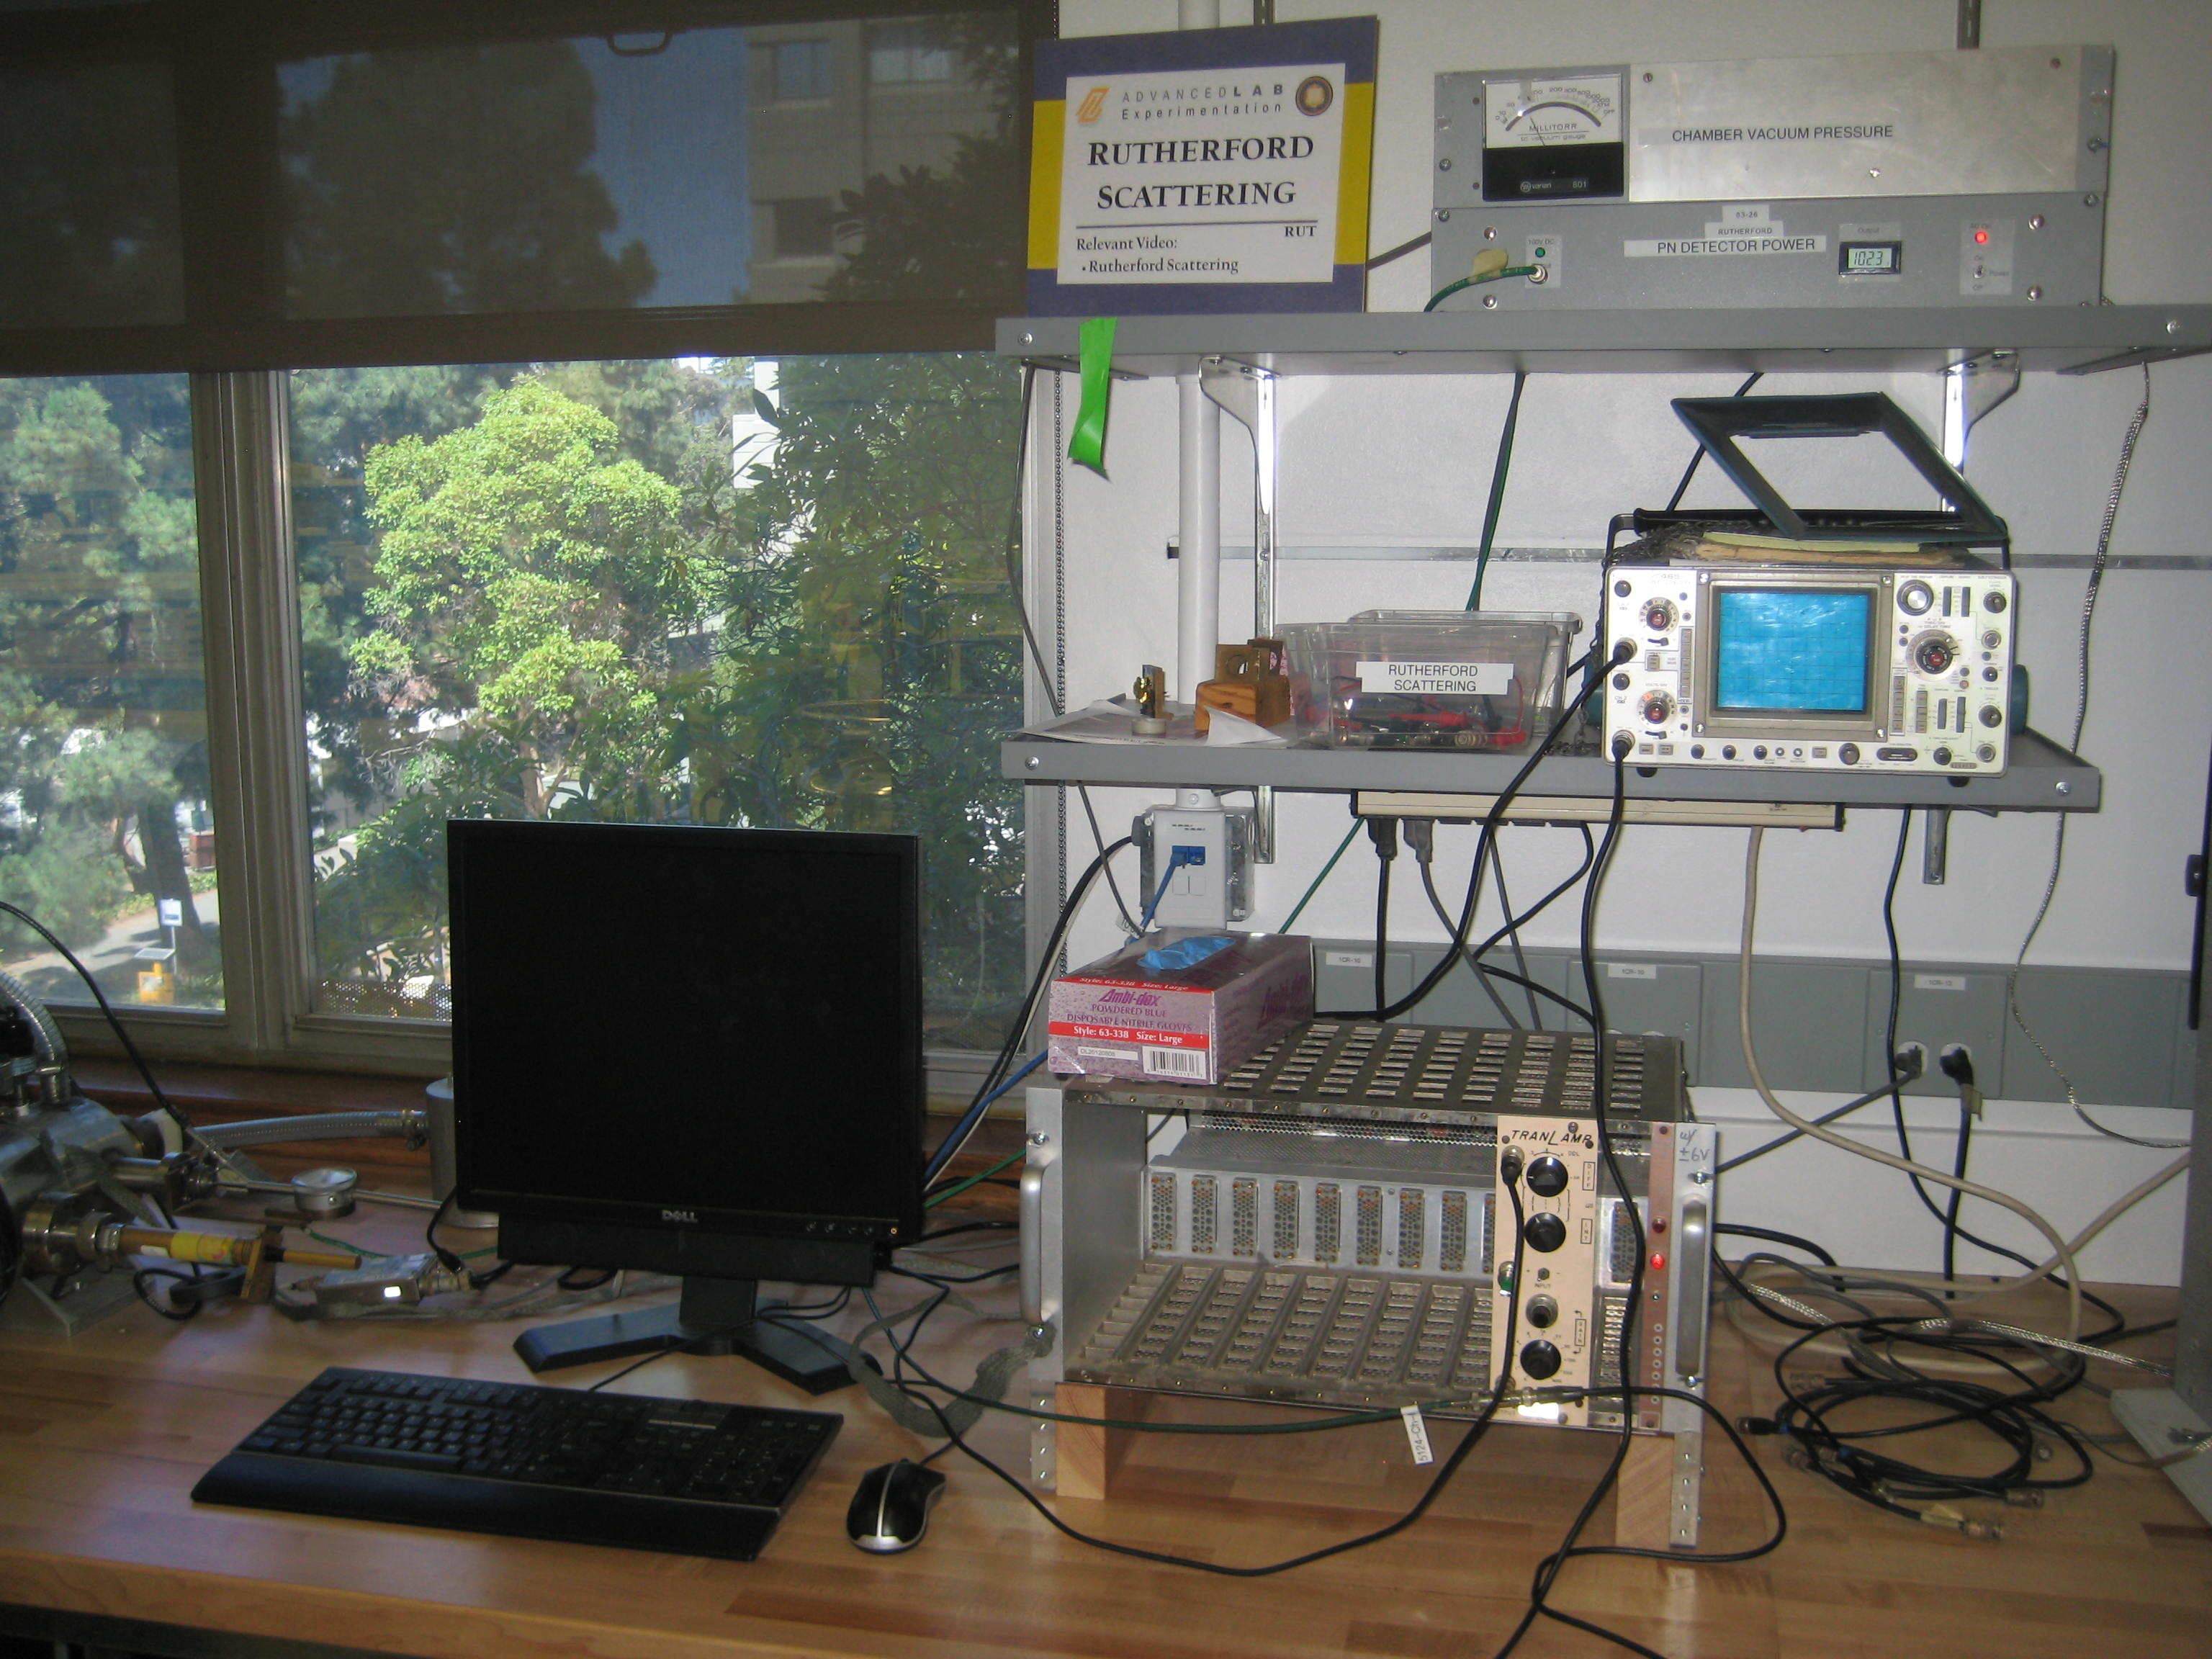
\includegraphics[width=0.33\linewidth,keepaspectratio]{images/RUT_3512.jpg}}
\href{http://experimentationlab.berkeley.edu/sites/default/files/images/RUT_Valve.jpg}{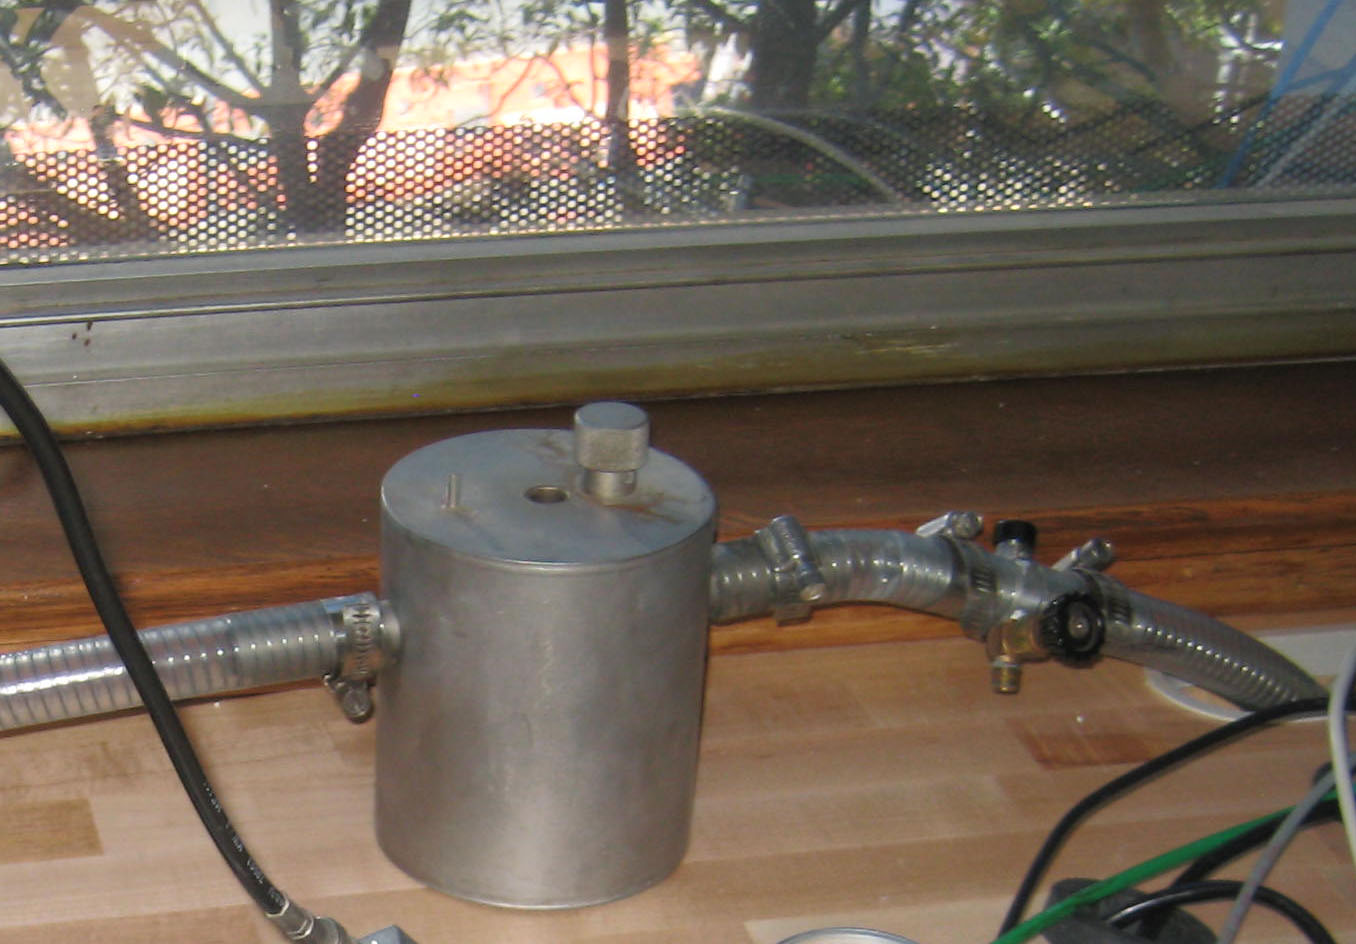
\includegraphics[width=0.33\linewidth,keepaspectratio]{images/RUT_Valve.jpg}}
\href{http://experimentationlab.berkeley.edu/sites/default/files/images/RUT_Chamber.jpg}{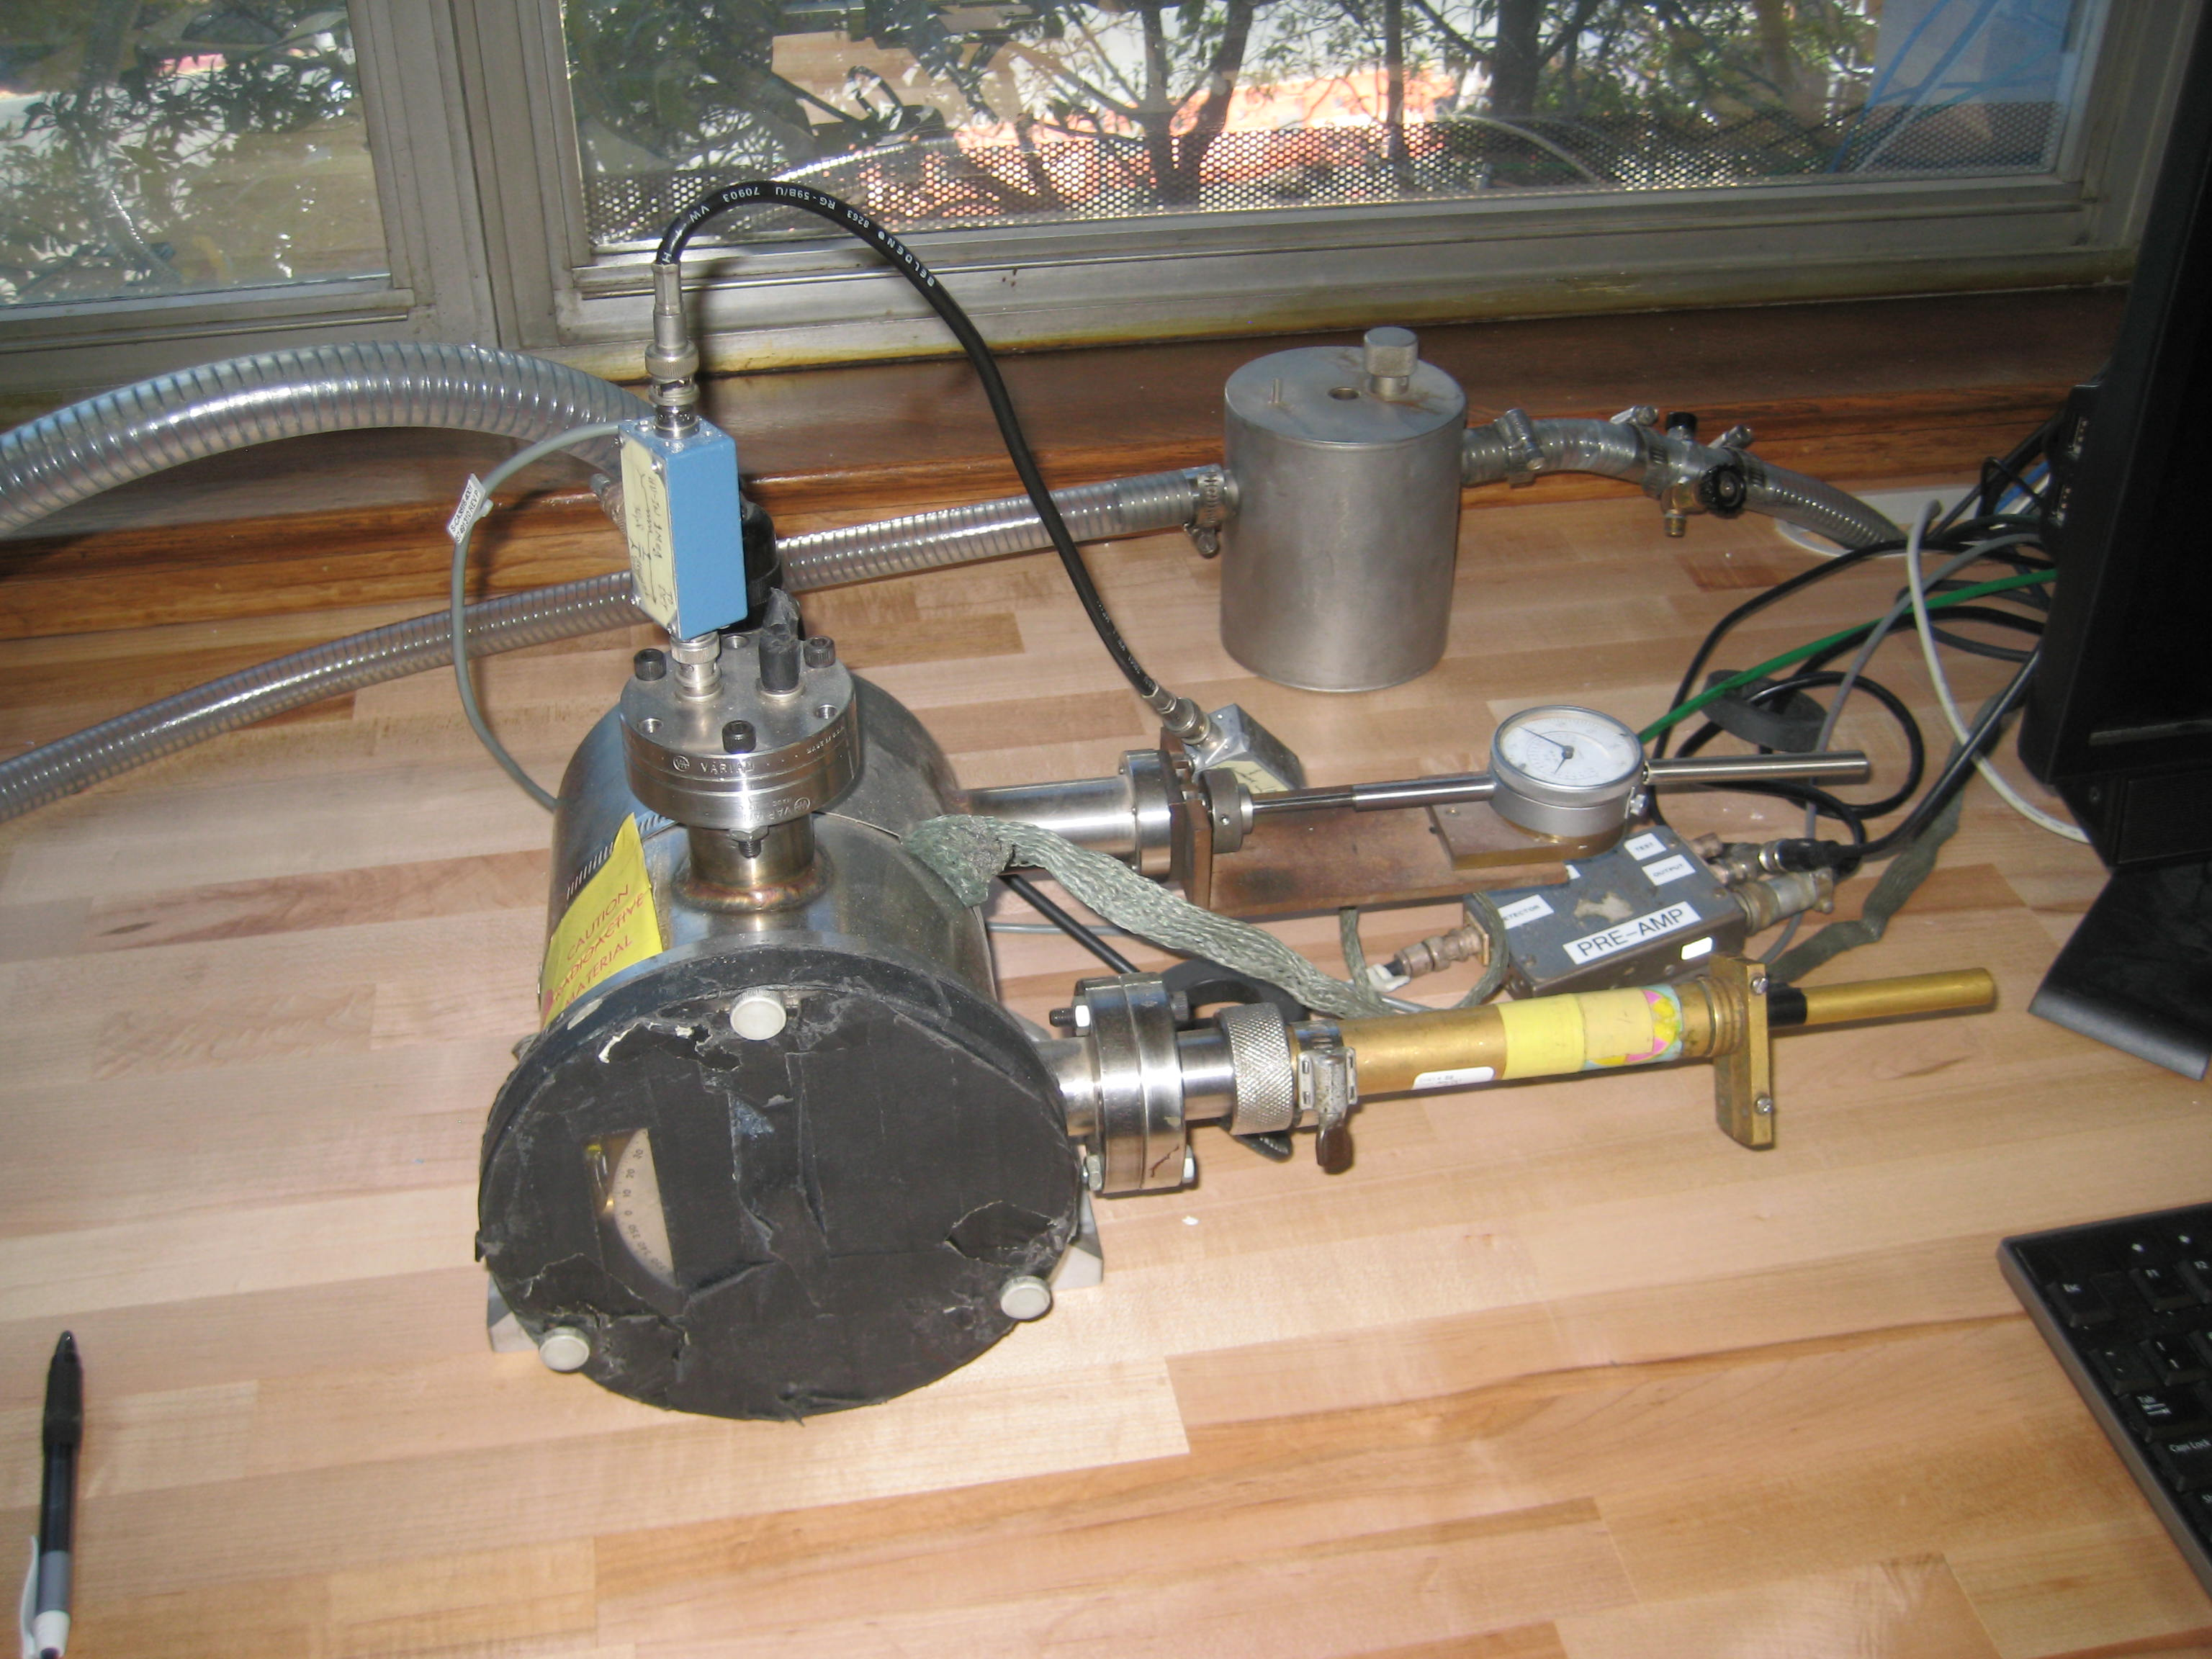
\includegraphics[width=0.33\linewidth,keepaspectratio]{images/RUT_Chamber.jpg}}

\section{Before the 1st Day of Lab and SOP's for this experiment}

\textbf{Complete the following before your experiment's scheduled start date:}

\begin{enumerate}
    \item View the \href{http://youtu.be/xHzzXiMEmaU}{\textbf{Rutherford Scattering video}}.

    \item View the \href{http://youtu.be/KHxtzF5pZZM}{\textbf{'\textbf{Radiation Safety Video'}}} After watching the video in the 111-Lab, get a pink Radiation Safety form from a 111-Lab staff person. Fill it out \& sign the form for getting a \textbf{Radiation Ring}.

    \item Now complete the Radiation Safety Training \href{http://experimentationlab.berkeley.edu/RadiationSafety}{\textbf{Radiation\_Safety}} \textbf{After completion of Training turn in all forms to Don Orlando.}

    \item \textbf{Check points} \emph{\textbf{are examination points that are placed in this lab where you must }}\emph{STOP and call a GSI or professor to make sure you understand what's expected. There could  be multiple check points throughout your lab so make sure you don't skip them since there is a \href{http://experimentationlab.berkeley.edurutcheckpoints}{\textbf{sign off sheet}}that must be turned in with your lab report. There are 3 Checkpoints in this lab.}

    \item Complete the \href{http://experimentationlab.berkeley.edu/RUTPreLab}{\textbf{RUT Pre Lab and Evaluation}} sheets. Print,  fill it out, then turn in your answers with the report. The Pre-Lab must be printed separately. Discuss the experiment and pre-lab questions with any faculty member or GSI and get it signed off by that faculty member or GSI. Turn in the signed pre-lab sheet with your lab report.

    \item View the \href{http://youtu.be/jR54387Wd6c}{\textbf{Introduction to Error Analysis video}} and \href{http://dev-physicsadv.pantheon.berkeley.edu/EAX}{\textbf{Error Analysis Notes}}.

    \item Read the Standard Operating Procedures (SOP) for this lab before starting \href{http://experimentationlab.berkeley.edu/sites/default/files/images/SOP\_3271\_Cs-137\_Na-22\_Co-60\_Mn-54\_Am-241\_Fe-55\_2014.pdf}{\textbf{SOP\_3271\_Cs-137\_Na-22\_Co-60\_Mn-54\_Am-241\_Fe-55\_2014}}.

    \item Last day of the experiment please fill out the \href{\ExperimentEvaluation}{\textbf{Experiment Evaluation}}

\end{enumerate}

\textbf{Suggested Reading:}

\begin{enumerate}
    \item A. C. Melissinos, Experiments in Modern Physic, 1966 \href{http://physics111.lib.berkeley.edu/Physics111/Reprints/RUT/RUT\%20\%20melissinos\%201966\%20rutherford\%20scattering.pdf}{\textbf{Melissions 1966}}

    \item R. D. Evans, \href{http://physics111.lib.berkeley.edu/Physics111/Reprints/R.D.Evans\%20Atomic\%20Nucleus/The\%20Atomic\%20Nucleus\%20Evans\%20full\%20text.pdf}{\textbf{The Atomic Nucleus}}. McGraw Hill (1972).

    \item ``\href{http://physics111.lib.berkeley.edu/Physics111/Reprints/RUT/03-Physics\_111\_Rutherford\_Scattering\_Experiment.pdf}{\textbf{Rutherford Experiment}}'', Physics 111-Lab Reprints in Physics Library.

    \item J.R. Comfort et al., ``\href{http://prola.aps.org/abstract/PR/v150/i1/p249\_1}{\textbf{Energy Loss and Straggling of Alpha Particles in Metal Foils}}''; Physical Review \textbf{150} (1966) 249. \href{http://physics111.lib.berkeley.edu/Physics111/Reprints/RUT/01-Energy\_Loss\_and\_Straggling.pdf}{\textbf{Searchable Page}}

    \item ``\href{http://physics111.lib.berkeley.edu/Physics111/Reprints/RUT/02-High\_Energy\_Particle\_Data.pdf}{\textbf{High-Energy Particle Data Volume II}}''; UC Radiation Lab: UCRL 2426, two pages.

    \item F.S. Goulding and D. Landis, ``\href{http://physics111.lib.berkeley.edu/Physics111/Reprints/RUT/04-Linear\_Amplifier.pdf}{\textbf{Linear Amplifier Gating \& Timing System}}'', Instrumentation Techniques in Nuclear Pulse Analysis, No. 1184, pp. 121-133.

    \item E. Rutherford, ``\href{http://physics111.lib.berkeley.edu/Physics111/Reprints/Beyer\_Foundations\%20of\%20Nuclear\%20Physics/The\%20scattering\%20of\%20a\%20and\%20b\%20particles\%20Rutherford.pdf}{\textbf{The Scattering of $ \alpha $ and $ \beta $ Particles}}'' and ``\href{http://physics111.lib.berkeley.edu/Physics111/Reprints/Beyer\_Foundations\%20of\%20Nuclear\%20Physics/Collision\%20of\%20a\%20particles\%20with\%20light\%20atoms\%20Rutherford.pdf}{\textbf{Collision of $ \alpha $ Particles by Light Atoms}}.'' by Matter and the Structures of the Atom, \emph{"Philosophical Magazine 21}, 699(1911). This article is conveniently reprinted in\emph{ Foundations of Nuclear Physics}, R.T. Beyer compiler., Dover Publications, New York, 1949. This reference appeals to students who are attracted to the historical aspects of the experiment. It contains references to other papers of historical importance.

\end{enumerate}

More

[\href{http://physics111.lib.berkeley.edu/Physics111/Reprints/RUT/RUT\_index.html}{\textbf{Physics 111 library site}}]

You should keep a laboratory notebook. The notebook should contain a detailed record of everything that was done and how/why it was done, as well as all of the data and analysis, also with plenty of how/why entries. This will aid you when you write your report.

\section{Objectives}

\begin{itemize}
    \item Learn what real experimental physics is about

    \item Learn the synergy between experimental and theoretical work

    \item Learn to use pieces of equipment that are commonly used in research

    \item Learn how measurements are performed, analyzed, and interpreted.

    \item Learn how to present your work and results

    \item Learn problem solving strategies

    \item Learn how to manage and organize your time

    \item 

\end{itemize}

\section{Introduction}

The Rutherford Scattering Experiment, in which α particles are scattered by a gold foil, is one of the most famous experiments ever performed in physics, because it demonstrated the validity of the \emph{nuclear} model for the atom and permitted a direct measurement of the nuclear charge. When alpha particles in a beam strike a gold foil and collide with individual gold nuclei, they are elastically scattered (no loss of energy). The collisions and the angles into which the the alpha particles are scattered are described by a model in which both the gold nuclei and the alpha particles act like charged spherical particles. The force of repulsion between them is described by the Coulomb's Law. The fraction of particles that are scattered into a particular solid angle at a given direction relative to the incoming beam is called the differential cross section and is given by

$ \frac{d\sigma}{d\Omega}=\left (\frac{Z_1Z_2e^2}{4E} \right )^2\sin^{-4}{\frac{\theta}{2}} $

where particle 1 is the helium nucleus (alpha particle), particle 2 is the gold nucleus, and E is the kinetic energy of the alpha particle. Of course there are electrons around each gold nucleus, but they are so light that the energetic alpha particles push them aside with a relatively small loss of energy.

In the experiment you will measure the relative numbers of alpha particles scattered as a function of scattering angle. You will observe the $sin^{-4}\frac{\theta}{2}$ dependence and from your data calculate the nuclear charge of gold .

\section{Equipment used in this experiment}

\begin{enumerate}
    \item Computer with National Instruments Digitizer card inside Used with the SoftScope and PHA-5124 programs.

    \item Radiation Safety video and dosiminator \href{http://experimentationlab.berkeley.edu/RadiationSafety}{\textbf{Radiation Safety}}

    \item Gloves

    \item \href{http://dev-physicsadv.pantheon.berkeley.edu/PHA-5124Program}{\textbf{PHA-5124 Program}}

    \item Tran-L-Amp Linear Amplifier

    \item \href{http://physics111.lib.berkeley.edu/Physics111/Reprints/RUT/RUT\_Detector\_018.JPG}{\textbf{PN Detector}} ( Do Not Touch this, it is very expensive)

    \item PN Detector Power supply and divider box

    \item \href{http://physics111.lib.berkeley.edu/Physics111/Reprints/RUT/Thermo\_Couple\_ionGauge.pdf}{\textbf{Vacuum ion gauge and pressure meter, Varian 801}}

    \item \href{http://physics111.lib.berkeley.edu/Physics111/Reprints/RUT/RUT\_Chamber\_017.JPG}{\textbf{Vacuum Chamber with Gold Foil Mount}}

    \item Radioactive source 241Am (130 microCi)

    \item Equipment

    \item Vacuum Pump and valve ( to open and close vacuum for chamber)

    \item Gold Foil and holder to be used in vacuum

\end{enumerate}

\section{Theory}

It is your responsibility to reproduce the necessary derivations for this experiment. Information on Rutherford scattering is usually first presented in Physics 7C. Detailed derivations are given in Physics 137A or Physics 105 courses and their associated texts. The recommended text for this course (Melissinos) is an excellent source for Rutherford Scattering. The bottom line is that you will need to find a relationship between what you measure - number of counts in a given time interval as a function of scattering angle - to the charge on the nucleus. The Rutherford formula and some algebra give $ Z=K\sqrt{N}\sin^2{\frac{\theta}{2}} $

where K is a constant depending upon the foil thickness, the strength of the source, the angular beam-width  and the counting time. N is the number of counts.

There are some models that are helpful in thinking about this experiment. The Rutherford scattering derivation assumes a single heavy charged spherical target and an α particle. But this experiment uses a gold foil, not single gold nuclei. What difference does this make to your experiment? It may help to think of the possible effects by breaking down the problem into two views. First, imagine the gold foil as an array of immobile gold atoms in space. Now remove the electrons from your picture. The remaining array of fixed bare nuclei is the first order experiment of Rutherford scattering. In this view you can see what it means to have a single scattering event or multiple scattering interactions.

To think of other effects in scattering, imagine the same gold foil array but remove the nuclei from your picture. What remains is a combination of fixed localized electrons (bound electrons) and an electron cloud (conduction electrons) in space. This picture greatly complicates the interpretation of the experimental data. α particles lose some energy in passing through this array and cloud of electrons. Because the electron-α particle interaction is actually quite complicated and difficult to treat, we create approximations for the interaction.

In our discussions we assumed that alpha particles have definite energies that you look up in a table. They do when emitted, but when we use them they do not, because the source is enclosed in a metallic capsule and the particles lose energy in passing through the capsule wall. Melissinos has a discussion on the loss of energy by alpha particles passing through matter. It is also true that they lose energy as they pass through the foil, as mentioned above. You must account for this when you analyze your data. The energy loss changes as the scattering angle changes. There is simply not enough time to go into detailed determinations of the energy loss. Instead, take the energy of the alpha particles for this experiment to be on average 3.77 MeV, and use this in your calculation of the nuclear charge of gold. You may wonder how Rutherford coped with this and other problems, since he had no sophisticated equipment. He had very much stronger radioactive sources, the sources were not shielded (the shields are a major source of energy loss), and he had people rather than a solid state detector and electronics to count scintillations, the flashes of light emitted when alpha particles strike a fluorescent screen used as a detector.

There are other reactions taking place, that we ignore: Cherenkov radiation, bremsstrahlung and inelastic nuclear interactions. If you have the time and interest, you can pursue the subject of energy losses in either of the two references given immediately below.

\begin{itemize}
    \item J.R. Comfort, et al., ``\href{http://physics111.lib.berkeley.edu/Physics111/Reprints/RUT/01-Energy\_Loss\_and\_Straggling.pdf}{\textbf{Energy Loss and Straggling of $ \alpha $ Particles in Metal Foils}}, ''Phys. Rev. 150, 249 (1966). Includes data for gold foils.

    \item J.H. Atkinson, Jr. and B.H. Wills, ``\href{http://physics111.lib.berkeley.edu/Physics111/Reprints/RUT/02-High\_Energy\_Particle\_Data.pdf}{\textbf{High Energy Data, Volume II,}}'' UCRL Report No. 2426 (1957). Page 35 of this report is a useful Range-Energy plot for $ \alpha $-particles of 4 to 10 MeV Kinetic energy. Gold is not included, but lead is.

\end{itemize}

\section{Experimental Overview}

The overall plan of the experiment is as follows. Alpha particles from a radioactive source called an alpha gun are made into a beam by two collimating apertures and directed toward a thin gold foil. Particles scattered by gold nuclei are counted by a detector placed at various angles to the beam direction. A histogram of particle counts vs. energy is made at each angle chosen. Even though nuclear scattering is elastic, some energy is always lost because of interactions with extra-nuclear electrons as mentioned above, and these losses are not exactly the same for every alpha particle. Consequently the histogram looks like a broad line rather than a delta function. The area under the line is proportional to the number of counts. With these numbers the angular scattering law mentioned above can be demonstrated, and the nuclear charge calculated.

The source of alpha particles is the isotope 241 of Americium at 130uCi. Its half-life is 458 years. The energies of emitted alpha particles are 5.49 MeV (86\%), 5.44 MeV (13\%), and 5.39 MeV (1.3\%). This also has a 59.6 Kev X-Ray which is used in the Compton experiment (neglecting other very infreguent α energies, all in the range of 5.55 to 4.8 Mev). The Americium is deposited as a thin layer on an aluminum foil located in the gun as shown below in Fig. 1. This deposit randomly flakes off so always ware your gloves.

\begin{figure}[h]
    \centering
    \href{http://experimentationlab.berkeley.edu/sites/default/files/images/RUTimage012.gif}{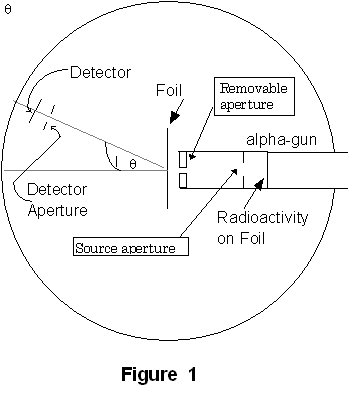
\includegraphics[width=0.5\linewidth]{images/RUTimage012.png}}
    \caption{}
    \label{fig:RUTimage012}
\end{figure}




Figure 1\section{Diagram of Vacuum Chamber}

The alpha particle gun and 2 pieces of gold foil 1 inch square are held in fixed positions when data are taken, ( you need to know the weight of each foil it should be in the log book) but the detector position can be moved at a constant radial distance from the foil. The particle beam is collimated by two apertures adjustable from the alpha gun. If necessary, changing the aperture separation is the easiest way to modify the collimation, since it can be changed without losing vacuum. It is also possible to remove the gun from the chamber and the removable aperture changed in size or removed entirely, \emph{\textbf{but do not touch the interior aperture}}. This aperture size is already measured and can be found in Fig. 3.

If we use a well collimated beam from the alpha-gun in order to have a well defined angular resolution, the total α-particle flux is weak so that counting rates at any appreciable scattering angle are extremely low. You will need a few all-night and week-end data collection runs. Plan accordingly.

The experiment is done in a \href{http://experimentationlab.berkeley.edu/sites/default/files/images/RUT\_Chamber.jpg}{\textbf{vacuum chamber and Valve}} because the range of alpha particles in air at atmospheric pressure is only a few cm.

\section{Procedure: getting started on Rutherford Scattering}

\begin{itemize}
    \item You must have a radiation ring and wear it when working near the apparatus, since there is an Americium-241 source which emits alpha particles and gamma rays. For safety, check the apparatus with a Geiger counter before you begin (counter usually kept at X-Ray or Gamma Ray experiments).

    \item Procedure for making of Gold Foil and mounting on brass holder \href{http://physics111.lib.berkeley.edu/Physics111/Reprints/RUT/Procedure\%20for\%20Making\%20Foils.pdf}{\textbf{Making of Gold Foil}}

\end{itemize}

\begin{enumerate}
    \item Familiarize yourself with the apparatus. Refer to Figs. 1, 2, 3. Start by removing the front cover from the chamber. Be aware of the angle cover piece, because \textbf{the detector is light sensitive}. \textbf{Keep it covered when using the experiment.} Put the screws somewhere where they won't be lost. Open the chamber and look at its construction. The detector is an extremely fragile device. There is a microscopically minute platinum wire between the attachment post and the evaporated gold surface of the detector. Break anything and you'll be out of commission for a week, minimum!


\begin{figure}[h]
    \centering
    \href{http://experimentationlab.berkeley.edu/sites/default/files/images/RUT13.jpg}{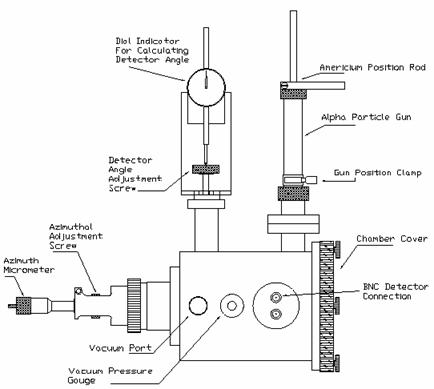
\includegraphics[width=0.5\linewidth]{images/RUT13.jpg}}
    \caption{}
    \label{fig:RUT13}
\end{figure}




	Figure 2: Diagram of apparatus. Top View

    \item Gently change the position of the detector using the \textbf{``detector angle adjusting screw''} shown in Fig. 2. Leave it at about zero degrees (protractor on front face of chamber). \textbf{Remember Do NOT change angle more than +30 to -30 degrees.} \textbf{NOTE: Keep window covered when in use.} Remove the foil holder from the chamber by grasping it firmly, pulling and wiggling it from side to side.


\begin{figure}[h]
    \centering
    \href{http://experimentationlab.berkeley.edu/sites/default/files/images/RUT14.gif}{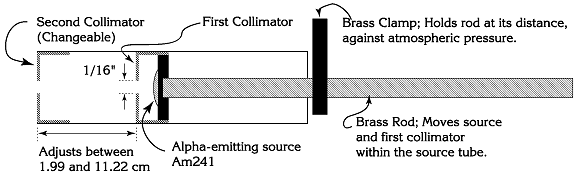
\includegraphics[width=0.5\linewidth]{images/RUT14.png}}
    \caption{}
    \label{fig:RUT14}
\end{figure}




Fig. 3: Alpha Gun
Remove the second aperture of the collimator, the one flush with the end of the gun, with the following procedure: loosen the brass rectangular clamp located at the end of the source tube on the brass rod (far right) of the alpha gun. Slowly push the rod into the tube-the second collimating aperture should fall out. Leave the rod positioned such that the first collimator is flush with the end of the source tube. Now loosen the brass ``O-ring'' clamp (nut) on the source tube, move the tube to the center of the chamber, and then retighten the clamp (finger tight). Also move the hose clamp on the source tube so that it is flush against the brass O-ring clamp, and tighten the hose clamp. It is important to retighten this clamp in the proper position after moving the gun. Otherwise atmospheric pressure on the outside will push the gun into the detector arm when the chamber is evacuated. Now make a run with no foil, non-collimated, point-blank, in order to find the beam flux, energy intensity profile and proper electronic settings.

    \item Pump down the chamber with the following procedure. Making sure that the cover is clean replace the chamber cover and tighten the thumb screws \textbf{by hand only}. Check to see if the cover is evenly seated on the vacuum chamber. Open the venting valve between the chamber and the pump on top of the bench near the chamber. Start the pump under the bench see switch for power \href{http://experimentationlab.berkeley.edu/sites/default/files/images/Pump\_Switch\_3535.jpg}{\textbf{Pump on/off Switch}} you then should here a hissing sound when the pump is running. The switch is located near the motor. Slowly close the valve the sound should go away. To open the chamber, reverse the process-slowly open the valve 1st and listen for the hissing sound, then turn off the pump. These precautions prevent shock waves from damaging the delicate gold foils, and minimize the amount of oil vapor from the pump entering the chamber. We are now going to use the scope to follow the signal through the electronics to set everything at proper levels. Do this carefully and ask questions if something does not seem right, but don't expect an Instructor to do your thinking for you and tell you what to do.

\end{enumerate}

\begin{equation}
    This Is a Checkpoint: Explain how the PN detector sends a signal to the computer. Also, without touching the PN detector, determine the solid angle of the detector. As stated below, the diameter is roughly 0.75 Inches.
\end{equation}
\section{Electronics see diagram here}

\begin{enumerate}
    \item Turn the electronics on. There are four switches to check: the master power switch in the lower right side of the Nim Bin, the then the Tran-L-Amp should be inside the Nim Bim rack.

    \item DETECTOR and PRE-AMP: The detector is a Silcon PN-junction with about 250 microns of gold on it. It has a bias of 50 volts at 4 microamps with a diameter of 0.75 inches. The detector receives its power through a voltage divider to get 50 volts from the 100 volt power supply in the rack. Take the output from the pre-amp (BNC coaxial cable) and feed it into the scope. Adjust the A TRIGGER LEVEL on the scope and see if you can obtain the positive pulse as shown in Fig. 5. You may have to increase the intensity of the trace, and put a hood on the oscilloscope to shut out room light. This pulse is the amplified signal from the detector. The positive voltage pulses represent the detected alpha particles, and the height of the pulses is proportional to the energy of the particles. Reconnect the output of the pre-amp to the AMP IN of the linear amplifier (PG1).

    \item Tran-L-Amp: This unit amplifies and shapes the unipolar pulse (unipolar means it goes up and comes down without crossing zero) from the pre-amp. The polarity knob must be set properly for the input pulses, should it be set to POSITIVE or NEGATIVE? To start with, also set the DIFF to 1.0, INT to 0.05, Coarse Gain to 100, and Vennier Gain to about 5.9. microseconds. For now, set the FINE GAIN at 1.75 (you should optimize the settings of this amplifier before starting taking serious data). Use the BNC cable to look at point PG2 ---the output of the Linear . You should see a signal like Figure. 5. Now use the Soft Scope program to view the signal at PG-2 look for a positive signal as seen below.

\end{enumerate}

\begin{figure}[h]
    \centering
    \href{http://experimentationlab.berkeley.edu/sites/default/files/images/350px-RUT_Soft_Scope.png}{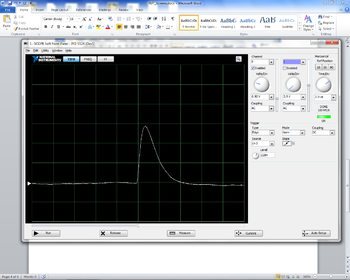
\includegraphics[width=0.5\linewidth]{images/350px-RUT_Soft_Scope.png}}
    \caption{}
    \label{fig:350px-RUT_Soft_Scope}
\end{figure}




\emph{Figure 5: Soft Scope display.} '\textbf{ Signal from PG-2 (Click on Picture to enlarge)}
\textbf{}\emph{\textbf{This Is a Checkpoint:}} Call a GSI or Professor over and show them all the signals you have found. Explain the signals.\section{PHA Setup and Operation}

\begin{enumerate}
    \item There is a LabView Program ICON on the computer desktop called ``PHA-5124''. Read \href{http://experimentationlab.berkeley.edu/PHA-5124Program}{\textbf{PHA-5124}} first. This program automates the data taking. Just double click on the Icon and take data. Before taking genuine data, determine the impact of the setting of the control parameters listed in the program. Make sure you understand each one and choose the proper setting for your measurement. Your data will be saved with a header and data such that it can be imported into Matlab or Excel. The dat will have time and day stamp on all of the files saved.

\end{enumerate}

\begin{figure}[h]
    \centering
    \href{http://experimentationlab.berkeley.edu/sites/default/files/images/350px-RUT_Spectrum_with_Foil.png}{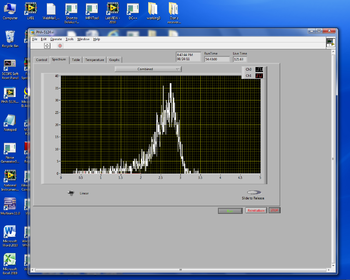
\includegraphics[width=0.5\linewidth]{images/350px-RUT_Spectrum_with_Foil.png}}
    \caption{}
    \label{fig:350px-RUT_Spectrum_with_Foil}
\end{figure}




\textbf{Spectrum With Gold Foil} (Click on Picture to Enlarge)\section{Handling gold foils}

[\href{http://physics111.lib.berkeley.edu/Physics111/Reprints/RUT/Procedure\%20for\%20Making\%20Foils.pdf}{\textbf{How to make and mount the Gold foils}}]

Since the scattering target is a gold foil, you need to know something about them.'\emph{\textbf{ '}}The foils are of very nonuniform thickness (Think holey swiss cheese) so you use double layers of gold leaf foil, each layer of which is about 10 milligrams by weight because of the holes and very fragile. Each pair of foils is fastened to a numbered holder by plastic tape. A weighed sample of each foil sheet is kept with the experiment. The weights should be recorded in the log book for each holder used. With them you can determine the surface density of each foil. In some cases this surface density is tabulated directly in the log book.

Handle the foils by the edges of the brass holder. Place foils carefully in the slotted repository when they are not in the chamber. The retaining fingers of the foil holder in the chamber are purposely loose so as not to abrade the tape. Keep them that way .

You are now READY TO GO ! ! !

\section{Data Collection (see Appendix on Error Analysis)}

\textbf{Error Analysis Notes} \href{http://experimentationlab.berkeley.edu/ErrorAnalysisNotes}{\textbf{Error Analysis Notes}}

Careful planning is essential if you want to complete this experiment. You can't possibly take all the data you need for a research-type project. As you take data, you will see where you have to make compromises. Talk them over with an instructor at every stage.

First you need to decide what you are going to measure. To do this, write down the equations you are going to use, identify those quantities you can measure (such as angle of scattering), those that are given (like the charge of the electron), and those that you want to determine. Then decide how you are going to make the measurements and what parameters you are going to vary to make the measurement an optimum for accuracy and time.

For example, you need to measure scattering angles. Therefore you need to establish the zero-degree position of the detector. How are you going to do this? Can you do it without the gold foil in place? Now is a good time to talk with an instructor, to be sure you are on the right track. Don't ask first - figure it out for yourself first, then explain to the instructor what you are going to do and why.

You will need to determine solid angles of the detector. You may want to change the solid angle for some measurements, by changing the aperture size.

The signals get weaker as the angles get larger. Think ahead, about how much time each data-taking run will require.

You may find it helpful to make a few trial runs, and analyze the data from them, before taking final measurements. If you are not doing the right thing, you want to find out about it immediately.

Finally, analyze your data, remembering that your goal is to observe the angular dependence of the Rutherford scattering formula, and to calculate the atomic number of gold.

One way to test the angular dependence of the differential scattering cross section is to fit a straight line to the data (review the formula and come up with a physical quantity based on the scattering angle that you should use for the x variable such that you end up with a linear function) and to determine the slope of this line by a least-squares fit. Follow the example given in Lyons, \emph{Data Analysis for Physical Science Students, }Chapter 2, especially Section 2.9, p. 63ff, in which is a worked example.

\section{Questions}

\begin{enumerate}
    \item At what scattering angles in your experiment will deviations from the Rutherford scattering law occur because of non-zero size of the nucleus?

    \item At what scattering angles will deviations occur because of screening of the nucleus by electrons?

    \item To what extent (be quantitative) do you expect alpha particles to experience multiple scattering in the foil?

    \item Last day of the experiment please fill out the \href{\ExperimentEvaluation}{\textbf{Experiment Evaluation}}

\end{enumerate}

\begin{equation}
     This is a Checkpoint: Show a Professor or GSi your spectrum taken over the weekend. Discuss if you think it is behaving as expected. Also discuss the questions above and how you will tackle them in your write up.
\end{equation}
\section{References}

\begin{enumerate}
    \item At the lab station there is an Americium 241 Data Sheet. Please take the time to read this and how to mount the Gold foils.

    \item Rutherford Detector \href{http://physics111.lib.berkeley.edu/Physics111/Reprints/RUT/RUT\_Detector\_018.JPG}{\textbf{Rutherford Detector}}

    \item Rutherford Chamber Alpha gun assembly \href{http://physics111.lib.berkeley.edu/Physics111/Reprints/RUT/RUT\_Chamber\_017.JPG}{\textbf{Chamber and Alpha Gun Assembly}}

    \item E.Segre, Nuclei and Particles 2nd.Ed., \href{http://physics111.lib.berkeley.edu/Physics111/Reprints/RUT/Scattering\%20From\%20Center\%20appendix\%20a.pdf}{\textbf{``Scattering from a Fixed Center of Force''}}

\end{enumerate}

There are many texts which incorporate a discussion of Rutherford Scattering at the junior level, such as Kennard, et al., Modern Physics, available in the Physics-Astronomy Library in Leconte.

Other reprints and reference materials can be found on the \href{http://physics111.lib.berkeley.edu/Physics111/Reprints/RUT/RUT\_index.html}{\textbf{Physics 111 Library Site}}

\end{document}